
% Please add the following required packages to your document preamble:
% \usepackage{multirow}

\begin{table*}[t]
\caption{Performances of state-of-the-art baselines and LLMs. Higher values indicate better performances.}
\label{exp_results}
\centering
\scalebox{0.65}{
\begin{tabular}{clcccccccccc}
\hline
\multicolumn{1}{c|}{\multirow{2}{*}{\textbf{Row}}} & \multicolumn{1}{c|}{\multirow{2}{*}{\textbf{Model}}} & \multicolumn{1}{c|}{\multirow{2}{*}{\textbf{Actor}}} & \multicolumn{1}{c|}{\multirow{2}{*}{\textbf{Action}}} & \multicolumn{2}{c|}{\textbf{Constraint}}              & \multicolumn{3}{c|}{\textbf{Gateway}}                                            & \multicolumn{3}{c}{\textbf{Flow}}                            \\ \cline{5-12} 
\multicolumn{1}{c|}{}                              & \multicolumn{1}{c|}{}                                & \multicolumn{1}{c|}{}                                & \multicolumn{1}{c|}{}                                 & \textbf{Data}  & \multicolumn{1}{c|}{\textbf{Action}} & \textbf{Exclusive} & \textbf{Inclusive} & \multicolumn{1}{c|}{\textbf{Parallel}} & \textbf{Sequence} & \textbf{Condition} & \textbf{Constraint} \\ \hline
\multicolumn{1}{c|}{1}                             & \multicolumn{1}{l|}{\citet{sonbol2023machine}}               & \multicolumn{1}{c|}{0.028}                           & \multicolumn{1}{c|}{0.308}                            & 0.213          & \multicolumn{1}{c|}{-}               & 0.485              & -                  & \multicolumn{1}{c|}{0.279}             & 0.056             & 0.047              & 0.017               \\ \cline{2-12} 
\multicolumn{1}{c|}{2}                             & \multicolumn{1}{l|}{\citet{neuberger2023beyond}}             & \multicolumn{1}{c|}{0.027}                           & \multicolumn{1}{c|}{0.276}                            & -              & \multicolumn{1}{c|}{-}               & 0.469              & -                  & \multicolumn{1}{c|}{0.337}             & 0.074             & 0.061              & -                   \\ \cline{2-12} 
\multicolumn{1}{c|}{3}                             & \multicolumn{1}{l|}{\citet{sholiq2022generating}}            & \multicolumn{1}{c|}{-}                               & \multicolumn{1}{c|}{0.387}                            & -              & \multicolumn{1}{c|}{-}               & 0.463              & -                  & \multicolumn{1}{c|}{0.198}             & 0.091             & 0.022              & -                   \\ \cline{2-12} 
\multicolumn{1}{c|}{4}                             & \multicolumn{1}{l|}{PET~\cite{bellan2023pet}}                             & \multicolumn{1}{c|}{0.085}                           & \multicolumn{1}{c|}{0.430}                            & 0.069          & \multicolumn{1}{c|}{-}               & \underline{0.493}              & -                  & \multicolumn{1}{c|}{-}                 & 0.164             & 0.026              & 0.000                    \\ \cline{2-12} 
\multicolumn{1}{c|}{5}                            & \multicolumn{1}{l|}{CIS~\cite{bellan2022leveraging}}                             & \multicolumn{1}{c|}{0.633}                           & \multicolumn{1}{c|}{0.639}                            & -              & \multicolumn{1}{c|}{-}               & 0.455              & -                  & \multicolumn{1}{c|}{-}                 & 0.203             & 0.157              & -                   \\ \hline
\multicolumn{1}{l|}{}                              & \multicolumn{1}{l|}{Flan-T5~\cite{chung2022scaling}}                         & \multicolumn{1}{c|}{}                                & \multicolumn{1}{c|}{}                                 &                & \multicolumn{1}{c|}{}                &                    &                    & \multicolumn{1}{c|}{}                  &                   &                    &                     \\
\multicolumn{1}{c|}{6}                             & \multicolumn{1}{l|}{\quad + Few-shot In-context Learning}               & \multicolumn{1}{c|}{0.206}                           & \multicolumn{1}{c|}{0.362}                            & -              & \multicolumn{1}{c|}{-}               & 0.376              & -                  & \multicolumn{1}{c|}{-}                 & 0.084             & 0.013              & -                   \\
\multicolumn{1}{c|}{7}                             & \multicolumn{1}{l|}{\quad + Supervised Fine-tuning}                     & \multicolumn{1}{c|}{\underline{0.659}}                           & \multicolumn{1}{c|}{\underline{0.684}}                            & 0.589          & \multicolumn{1}{c|}{\underline{0.366}}           & 0.419              & 0.045              & \multicolumn{1}{c|}{\underline{0.393}}             & 0.395             & \underline{0.168}              & 0.363               \\ \hline
\multicolumn{1}{l|}{}                             & \multicolumn{1}{l|}{ChatGPT~\cite{ouyang2022training}}                         &  \multicolumn{1}{c|}{}                                 & \multicolumn{1}{c|}{}                                 &                & \multicolumn{1}{c|}{}                &                    &                    & \multicolumn{1}{c|}{}                  &                   &                    &                     \\

\multicolumn{1}{c|}{8}                             & \multicolumn{1}{l|}{\quad + Few-shot In-context Learning} &\multicolumn{1}{c|}{0.625}                           & \multicolumn{1}{c|}{0.681}                            & \underline{0.687}          & \multicolumn{1}{c|}{0.286}           & 0.477              & \textbf{0.173}     & \multicolumn{1}{c|}{0.388}             & \underline{0.408}             & 0.158              & 0.\underline{444}               \\ \hline
\multicolumn{1}{l|}{}                              & \multicolumn{1}{l|}{Llama2~\cite{touvron2023llama}}                          & \multicolumn{1}{c|}{}                                & \multicolumn{1}{c|}{}                                 &                & \multicolumn{1}{c|}{}                &                    &                    & \multicolumn{1}{c|}{}                  &                   &                    &                     \\
\multicolumn{1}{c|}{9}                             & \multicolumn{1}{l|}{\quad + Few-shot In-context Learning}               & \multicolumn{1}{c|}{0.502}                           & \multicolumn{1}{c|}{0.573}                            & 0.357          & \multicolumn{1}{c|}{0.049}           & 0.446              & 0.067              & \multicolumn{1}{c|}{0.128}             & 0.193             & 0.107              & 0.201               \\
\multicolumn{1}{c|}{10}                            & \multicolumn{1}{l|}{\quad + Supervised Fine-tuning}                     & \multicolumn{1}{c|}{\textbf{0.674}}                  & \multicolumn{1}{c|}{\textbf{0.744}}                   & \textbf{0.779} & \multicolumn{1}{c|}{\textbf{0.499}}  & \textbf{0.554}     & \underline{0.090}              & \multicolumn{1}{c|}{\textbf{0.398}}    & \textbf{0.478}    & \textbf{0.319}     & \textbf{0.467}      \\ \hline
\multicolumn{12}{l}{\small * The best results are marked in bold, and the second-best results are marked with underlines.}                                                                                                                                                                                                                                                                                                                 
\end{tabular}
}
\vspace{5pt}
\end{table*}

% ~\citet{sonbol2023machine}
% ~\citet{neuberger2023beyond}
% ~\citet{bellan2022leveraging}
% PET~\citet{bellan2023pet}
% CIS~\citet{bellan2022leveraging}


% \begin{table*}[t]
% \caption{Performances of state-of-the-art baselines and LLMs. Higher values indicate better performances.}
% \label{exp_results}
% \centering
% \scalebox{0.68}{
% \begin{tabular}{l|c|c|cc|ccc|cccll}
% \cline{1-11}
% \multicolumn{1}{c|}{\multirow{2}{*}{\textbf{Model}}}                                                             & \multirow{2}{*}{\textbf{Actor}}             & \multirow{2}{*}{\textbf{Action}}            & \multicolumn{2}{c|}{\textbf{Constraint}}                                                                                           & \multicolumn{3}{c|}{\textbf{Gateway}}                                                                                   & \multicolumn{3}{c}{\textbf{Flow}}                                                                                                                                                                           & \multicolumn{1}{c}{} & \multicolumn{1}{c}{} \\ \cline{4-11}
% \multicolumn{1}{c|}{}                                                                                   &                                    &                                    & \textbf{\makecell{Data}} & \textbf{\makecell{Action}} & \textbf{Exclusive} & \textbf{Inclusive} & \textbf{Parallel} & \textbf{\makecell{Sequence}} & \textbf{\makecell{Condition}} & \textbf{\makecell{Constraint}} &                      &                      \\  \cline{1-11}
% [1] \citet{sonbol2023machine}                                                                         & 0.028                              & 0.308                              & 0.213                                                      & -                                                          & 0.485                               & -                                 & 0.279                              & 0.056                                                          & 0.047                                                           & 0.017                                                            &                      &                      \\
% \cline{1-11}
% [2] \citet{neuberger2023beyond}                                                                              & 0.027                              & 0.276                              & -                                                        & -                                                          & 0.469                               & -                                 & 0.337                              & 0.074                                                          & 0.061                                                           & -                                                              &                      &                      \\ 
% \cline{1-11}
% [3] \citet{sholiq2022generating}                                                                               & -                                & 0.387                              & -                                                        & -                                                          & 0.463                               & -                                 & 0.198                              & 0.091                                                          & 0.022                                                           & -                                                              &                      &                      \\
% \cline{1-11}
% [4] CIS~\cite{bellan2022leveraging}                                                                                      & 0.633                              & 0.639                              & -                                                        & -                                                          & 0.455                               & -                                 & -                                & 0.203                                                          & 0.157                                                           & -                                                              &                      &                      \\
% \cline{1-11}
% [5] PET~\cite{bellan2023pet}                                                                                      & 0.085                              & 0.430                              & 0.069                                                      & -                                                          & \underline{0.493}  & -                                 & -                                & 0.164                                                          & 0.026                                                           & -                                                              &                      &                      \\ 
% \cline{1-11}
% \cline{1-11}

% Flan-T5~\cite{chung2022scaling} &&&&&&&&&&& & \\
 
% [6] \quad + Few-shot Learning& 0.206 & 0.362 & - & - & 0.376 & - & - & 0.084 & 0.013 & - &                    &                      \\ 

% [7] \quad + Fine-tuning& \underline{0.659} & \underline{0.684} & 0.589                                                      & \underline{0.366}                           & 0.419                               & 0.045                               & \underline{0.393} & 0.395                                                          & \underline{0.168}                              & 0.363                                                            &                      &                      \\ 
%  \cline{1-11}
% [8] ChatGPT~\cite{ouyang2022training}                                                                                 & 0.625                              & 0.681                              & \underline{0.687}                         & 0.286                                                        & 0.477                               & \textbf{0.173}     & 0.388                              & \underline{0.408}                             & 0.158                                                           & \underline{0.444}                               &                      &                      \\
%  \cline{1-11}
%  Llama2~\cite{touvron2023llama}&&&&&&&&&&& & \\

% [9] \quad + Few-shot Learning& 0.502                              & 0.573                              & 0.357                                                      & 0.049                                                        & 0.446                               & 0.067                               & 0.128                              & 0.193                                                          & 0.107                                                           & 0.201                                                            &                      &                      \\

% [10] \quad + Fine-tuning                                                                     & \textbf{0.674}    & \textbf{0.744}    & \textbf{0.779}                            & \textbf{0.499}                              & \textbf{0.554}     & \underline{0.090}  & \textbf{0.398}    & \textbf{0.478}                                & \textbf{0.319}                                 & \textbf{0.467}                                  &                      &                      \\ 
% \cline{1-11}
% \multicolumn{11}{l}{\small * The best results are marked in bold, and the second-best results are marked with underlines.} &&\\
% \end{tabular}}
% \end{table*}

% \begin{table*}[!th]
% \caption{Experimental results of the baseline models. The best results are represented in bold, and the second best results are highlighted with an underline. For simplicity, we use ``XOR'', ``OR'' and ``AND'' as abbreviations for exclusive, inclusive and parallel gateways respectively.}
% \label{exp_results}
% \centering
% \scalebox{0.72}{
% \begin{tabular}{l|c|ccc|cc|ccc|c}
% \hline
% \multicolumn{1}{c|}{\multirow{3}{*}{\textbf{Model}}} & \multirow{3}{*}{\textbf{Action}} & \multicolumn{3}{c|}{\textbf{Gateway}}               & \multicolumn{2}{c|}{\textbf{Constraint}}            & \multicolumn{3}{c|}{\textbf{Flow}}                                       & \multirow{3}{*}{\textbf{Actor}} \\ \cline{3-10}
% \multicolumn{1}{c|}{}                                &                                  & \textbf{XOR}    & \textbf{OR}     & \textbf{AND}    & \textbf{\makecell{Data\\Constraint}} & \textbf{\makecell{Action\\Constraint}} & \textbf{\makecell{Sequence\\Flow}} & \textbf{\makecell{Condition\\Flow}} & \textbf{\makecell{Constraint\\Flow}} &                                 \\ \hline
% \uppercase\expandafter{\romannumeral1}. Pipeline Based                                       &                                  &                 &                 &                 &                         &                           & \textbf{}             & \textbf{}              &                         &                                 \\
% \ Translation Like                                     & 0.308                           & 0.485          &---              & 0.279          & 0.213                  &---                         & 0.056                & 0.047                 & 0.017                  & 0.028                          \\
% \ Beyond Rule                                          & 0.276                           & 0.469          &---              & 0.337          &---                      &---                        & 0.074                & 0.061                 &---                      & 0.027                          \\ \hline
% \uppercase\expandafter{\romannumeral2}. Elements Linking                                     &                                  &                 &                 &                 &                         &                           &                       &                        &                         &                                 \\
% \ Fact Types                                           & 0.387                           & 0.463          &---              & 0.198          &---                      &---                        & 0.091                & 0.022                &---                      &---                              \\
% \ PET                                                  & 0.430                           & \underline{0.493}          &---              &---              & 0.069                  &---                        & 0.164                & 0.026                 &---                      & 0.085                          \\
% \ CIS                                                  & 0.639                           & 0.455          &---              &---              &---                      &---                        & 0.203                & 0.157                 &---                      & 0.633                          \\ \hline
% \uppercase\expandafter{\romannumeral3}. End to End                                           &                                  &                 &                 &                 &                         &                           &                       &                        &                         &                                 \\
% \ Flan-T5 fine-tuned                                   & \underline{0.684}                           & 0.419          & 0.045          & \underline{0.393}          & 0.589                  & \underline{0.366}                    & 0.395                & \underline{0.168}                 & 0.363                  & \underline{0.659}                          \\
% \ ChatGPT                                              & 0.681                           & 0.477          & \textbf{0.173} & 0.388          & \underline{0.687}                  & 0.286                    & \underline{0.408}                & 0.158                 & \underline{0.444}                  & 0.625                          \\
% \ Llama2 few-shot                                      & 0.573                           & 0.446          & 0.067          & 0.128          & 0.357                  & 0.049                    & 0.193                & 0.107                 & 0.201                  & 0.502                          \\
% \ Llama2 fine-tuned                                    & \textbf{0.744}                  & \textbf{0.554} & \underline{0.090}          & \textbf{0.398} & \textbf{0.779}         & \textbf{0.499}           & \textbf{0.478}       & \textbf{0.319}        & \textbf{0.467}         & \textbf{0.674} \\ \hline          
% \end{tabular}
% }
% \end{table*}
% \begin{table*}[!th]
% \caption{Experimental results of the baseline models. The best results are represented in bold, and the second best results are highlighted with an underline. For simplicity, we use ``XOR'', ``OR'' and ``AND'' as abbreviations for exclusive, inclusive and parallel gateways respectively.}
% \label{exp_results}
% \centering
% \scalebox{0.72}{
% \begin{tabular}{l|c|ccc|cc|ccc|c}
% \hline
% \multicolumn{1}{c|}{\multirow{3}{*}{\textbf{Model}}} & \multirow{3}{*}{\textbf{Action}} & \multicolumn{3}{c|}{\textbf{Gateway}}               & \multicolumn{2}{c|}{\textbf{Constraint}}            & \multicolumn{3}{c|}{\textbf{Flow}}                                       & \multirow{3}{*}{\textbf{Actor}} \\ \cline{3-10}
% \multicolumn{1}{c|}{}                                &                                  & \textbf{XOR}    & \textbf{OR}     & \textbf{AND}    & \textbf{\makecell{Data\\Constraint}} & \textbf{\makecell{Action\\Constraint}} & \textbf{\makecell{Sequence\\Flow}} & \textbf{\makecell{Condition\\Flow}} & \textbf{\makecell{Constraint\\Flow}} &                                 \\ \hline
% \uppercase\expandafter{\romannumeral1}. Pipeline Based                                       &                                  &                 &                 &                 &                         &                           & \textbf{}             & \textbf{}              &                         &                                 \\
% Translation Like                                     & 0.3079                           & 0.4848          &---              & 0.2786          & 0.2133                  &---                        & 0.0558                & 0.0468                 & 0.0172                  & 0.0276                          \\
% Beyond Rule                                          & 0.2757                           & 0.4685          &---              & 0.3369          &---                      &---                        & 0.0744                & 0.0611                 &---                      & 0.0266                          \\ \hline
% \uppercase\expandafter{\romannumeral2}. Elements Linking                                     &                                  &                 &                 &                 &                         &                           &                       &                        &                         &                                 \\
% Fact Types                                           & 0.3874                           & 0.4633          &---              & 0.1983          &---                      &---                        & 0.0910                & 0.0223                 &---                      &---                              \\
% PET                                                  & 0.4297                           & \underline{0.4932}          &---              &---              & 0.0689                  &---                        & 0.1640                & 0.0257                 &---                      & 0.0846                          \\
% CIS                                                  & 0.6393                           & 0.4549          &---              &---              &---                      &---                         & 0.2034                & 0.1574                 &---                      & 0.6326                          \\ \hline
% \uppercase\expandafter{\romannumeral3}. End to End                                           &                                  &                 &                 &                 &                         &                           &                       &                        &                         &                                 \\
% Flan-T5 fine-tuned                                   & \underline{0.6843}                           & 0.4188          & 0.0449          & \underline{0.3932}          & 0.5887                  & \underline{0.3661}                    & 0.3952                & \underline{0.1678}                 & 0.3626                  & \underline{0.6589}                          \\
% ChatGPT                                              & 0.6812                           & 0.4768          & \textbf{0.1729} & 0.3878          & \underline{0.6873}                  & 0.2859                    & \underline{0.4078}                & 0.1581                 & \underline{0.4442}                  & 0.6245                          \\
% Llama2 few-shot                                      & 0.5725                           & 0.4459          & 0.0672          & 0.1284          & 0.3571                  & 0.0492                    & 0.1927                & 0.1074                 & 0.2005                  & 0.5020                          \\
% Llama2 fine-tuned                                    & \textbf{0.7439}                  & \textbf{0.5539} & \underline{0.0900}          & \textbf{0.3979} & \textbf{0.7788}         & \textbf{0.4991}           & \textbf{0.4777}       & \textbf{0.3190}        & \textbf{0.4669}         & \textbf{0.6742}                
% \end{tabular}
% }
% \end{table*}

% \uppercase\expandafter{\romannumeral1}



\section{Experiments}
% To comprehensively evaluate the performance of existing studies, we select several representative models that perform best in current datasets from recent studies. 
% Meanwhile, we select the emerging large language models that perform well in various fields to explore whether these powerful large models can help to solve this task well. 

% It should be noticed that, due to the difficulty in generating procedure graph directly by the model, we use a dot language based textual representation~\cite{grohs2023large} in the form of ``NODE -> (condition) NODE'' as the equivalent representation of the graph structure. This can greatly facilitate our exploration of this task through the paradigm of text generation. 


We conduct systematic experiments to answer the two research questions: 
(1) \textit{whether the existing studies have well solved the automated extraction of procedural graphs from procedural documents}; (2) \textit{whether the emerging large language models can bring new opportunities to this task}. 

\subsection{Experimental Setup}

\subsubsection{Baselines}
% V1
% We select several representative models that perform best in current datasets to measure the performance of existing methods. And we also aim to explore the perform of the emerging large language models. 
% The selected baseline models can be divided into three categories. They are listed as follows:

% \begin{enumerate}[label=\Roman*., itemsep=3pt,topsep=3pt,parsep=0pt,leftmargin=16pt]
%     \item \textbf{Pipeline Based}:
%     \begin{enumerate}[itemsep=0pt,topsep=1pt,parsep=0pt,leftmargin=1pt]
%         \item[--] \textbf{Translation Like}: a machine translation like pipeline based on syntactic analysis, semantic analysis and transformation between source text and the target procedural graph~\cite{sonbol2023machine}. 
%         \item[--] \textbf{Beyond Rule}: a three-step pipeline to identify nodes of the procedural graphs with information extraction technologies and construct their relations by hand-written rules~\cite{neuberger2023beyond}. 
%     \end{enumerate}
    
%     \item \textbf{Elements Linking}:
%     \begin{enumerate}[itemsep=0pt,topsep=2pt,parsep=0pt,leftmargin=1pt]
%         \item[--] \textbf{Fact Types}: extracting elements on the procedural graphs based on an intermediate representation named fact types and linking them by hand-written rules~\cite{sholiq2022generating}. 
%         \item[--] \textbf{PET}: Conditional Random Fields based approach to support elements extraction and linking for the procedural graphs~\cite{bellan2022pet}. 
%         \item[--] \textbf{CIS}: using pre-trained language model to extract elements of the procedural graphs with in-context learning~\cite{bellan2022leveraging}. 
%     \end{enumerate}
    
%     \item \textbf{End to End}:
%     \begin{enumerate}[itemsep=0pt,topsep=1pt,parsep=0pt,leftmargin=1pt]
%         \item[--] \textbf{Flan-T5}: sequence-to-sequence language model trained on instruction data with a large scale number of downstream tasks~\cite{chung2022scaling}. 
%         \item[--] \textbf{Llama2}: generative text model that adapts to human preferences through supervised fine-tuning and reinforcement learning with human feedback~\cite{touvron2023llama}. 
%         \item[--] \textbf{ChatGPT}: a large language model with the ability to generate coherent responses through conversation~\cite{ouyang2022training}. 
%     \end{enumerate}
    
% \end{enumerate}

% V2
We select several state-of-the-art solutions to measure the performance of existing studies. And we also aim to explore the performance of the emerging large language models. 
The selected baseline models can be divided into three categories, listed as follows:

\paragraph{Pipeline Based}
(1) \textbf{Translation Like}: a machine translation like pipeline based on syntactic analysis, semantic analysis and transformation between source text and the target procedural graph~\cite{sonbol2023machine}. 
(2) \textbf{Beyond Rule}: a three-step pipeline to extract actions and gateways with information extraction technologies and construct the procedural graphs by hand-written rules~\cite{neuberger2023beyond}. 

\paragraph{Elements Linking}
(1) \textbf{Fact Types}: extract elements on the procedural graphs based on an intermediate representation named fact types and link them by hand-written rules~\cite{sholiq2022generating}. 
(2) \textbf{PET}: Conditional Random Fields based approach to support elements extraction and linking for the procedural graphs~\cite{bellan2022pet}. 
(3) \textbf{CIS}: use pre-trained language model to extract individual actions and conditions for their execution~\cite{bellan2022leveraging}. 

\paragraph{End to End}
(1) \textbf{Flan-T5}: sequence-to-sequence language model pre-trained with a large scale number of downstream tasks~\cite{chung2022scaling}. 
(2) \textbf{ChatGPT}: a large language model that can utilize in-context learning to facilitate procedural graphs extraction with designed instruction and a few examples~\cite{ouyang2022training}. 
(3) \textbf{Llama2}: a large language model capable of in-context learning and can be further fine-tuned on our dataset~\cite{touvron2023llama}. 


\subsubsection{Metric}
% Following current studies~\cite{Bellan2021ProcessEF, bellan2022pet, neuberger2023beyond}, we adopt standard F-1 score to evaluate the extracted procedural graphs in terms of nodes, edges, and actors. 
% For nodes evaluation, a node is considered successfully extracted only if the type and text of words of the node exactly match the type and text of words of the gold-standard label. After successfully matching the action nodes predicted by the model, we further consider the match of the actors for each action node. 
% For edge evaluation, an edge is considered successfully extracted only if the two nodes connected by the edge can exactly match the corresponding two nodes connected by the edge of the gold-standard label. 
% In addition, for edges connecting exclusive or inclusive gateways with other nodes, the conditions between extracted and gold-standard edges must also be matched. To avoid the disturbance of words' different morphology and tenses, we compare the stems of words of different texts and ignore the prepositions for soft comparison. 

% We adopt standard F-1 score to evaluate the extracted procedural graphs in terms of nodes, edges, and actors following current studies~\cite{bellan2022pet, neuberger2023beyond}. 
% A node is successfully extracted only if its type and text~(for actions and constraints) exactly match the gold-standard label. After matching the predicted action nodes, we then consider the match of actor for each action node. 
% An edge is successfully extracted only if its connected nodes and condition~(for edges connecting exclusive or inclusive gateways) exactly match those of the gold-standard label. 
% To avoid the disturbance of preposition words and words' morphology and tenses, we compare the stems of words of different texts. For example, ``submits the order'' is considered to be a successful match with ``submit the order''. 

The extraction of optimal procedural graphs requires not only identifying actions in the document, but more importantly: (1) using suitable gateways to represent the non-sequential execution of actions; (2) identifying vital constraints and actors of corresponding actions; (3) using flows to link all actions, gateways and constraints to form a complete procedural graph. 
Hence, we use BLEU~\cite{papineni2002bleu} metric to evaluate the model's accuracy in identifying actions, constraints, and actors. 
Then we use standard F1-score to evaluate the model's accuracy in using suitable gateways to represent non-sequential actions execution and correctly linking elements in procedural graphs using flows. 

Note that a flow is considered correctly extracted if its type and connected elements match those of the gold label. For a soft comparison, an element is considered matched with the gold label if its type matches the gold label and the BLEU score $\geq 0.5$~(gateways only require type match). 
For conditional flow, we compute the BLEU score between its condition and the gold label's condition if a condition flow in the gold label can be matched. 

\subsubsection{Implementation Details}
We divide our constructed dataset into three subsets: train set(1697 samples), validation set(543 samples), and test set(1154 samples), and evaluate the performance of all models uniformly on the test set. Pipeline Based and Elements Linking models do not require training data, except for PET trained on its own data. Therefore, we evaluate these models on our test set according to the original papers' setting. 
End to End models utilize our train set to fine-tune the model or construct examples for in-context learning, and use the validation set for model selection~\cite{raschka2018model}. 
To make good use of the capabilities of LLMs, we adopt the Chain-of-thought~(CoT)~\cite{wei2022chain} strategy to guide the inference process of extracting procedural graphs for the model, especially for the extraction of non-sequential actions. See Appx.~\ref{app:Experiments} for more details. 

\subsection{Results and Analysis}
% The performance of our proposed framework and baseline models are shown in Table~\ref{exp_results}. 
% Experimental results show the superiority of our proposed framework compared to other models, especially for the extraction of gateways. This demonstrates that our proposed framework can facilitate the model to better understand the complex branches in the documents and use correct gateways to represent them. 
% Additionally, we aim to answer the two research questions: 

\subsubsection{Performance of Existing Studies}
% V1
% Experimental results demonstrate that the existing studies are far from solving this task well. In fact, the existing studies neglects important inclusive gateways and the necessary factual knowledge in the procedural graphs, resulting in poor performance. 
% Additionally, we have the following observations:
% 1) Traditional Pipeline Based and Elements Linking methods generally perform worse than End to End methods. This is because the hand-written rules used by these methods can not cover various procedures in the real world, resulting in poor generalization. 
% 2) Due to the heavy reliance on syntax and semantic parsing, traditional methods are difficult to accurately extract action nodes from the procedural documents, as the complex expressions of the actions in the document are difficult to be fully extracted through parsing results and hand-written rules. 
% 3) The extraction of actors of corresponding action nodes is extremely challenging for traditional methods, as the expressions of actors in procedural documents are variable, making it difficult to extract the actors by rules. 
% 4) For Elements Linking baselines, CIS achieves better performance for action extraction with the help of pre-trained large model, but performs worse for exclusive gateway extraction than other two methods. This is because pre-trained large models are capable of understanding the surface semantic information of the text, but are not good at understand complex branches, which indicates that the combination of large models and insightful heuristic rules may be a way to solve this task. 

% V2
As shown in Table~\ref{exp_results}, 
experimental results demonstrate that existing studies are far from solving this task well as they perform poorly for the extraction of nearly all elements and neglect important gateways and constraints. 
Additionally, we have the following observations:
1) Traditional methods generally perform worse than End to End methods because hand-written rules used by them can not cover various procedures, resulting in poor generalization. 
2) Due to the heavy reliance on syntax and semantic parsing, traditional methods are difficult to accurately extract actions, constraints and actors from the procedural documents, as the complex expressions in documents are difficult to extract through parsing results and hand-written rules. 
3) For Elements Linking baselines, CIS achieves better performance for actions extraction with the help of large language model, but performs worse for gateways extraction than other two methods. This is because LLM is capable of understanding the surface semantic information of the text, but is not good at understand non-sequential execution of actions, which indicates that the combination of LLM and insightful heuristic rules may be a way to solve this task well. 

\begin{figure*}[!t]
    \centering
    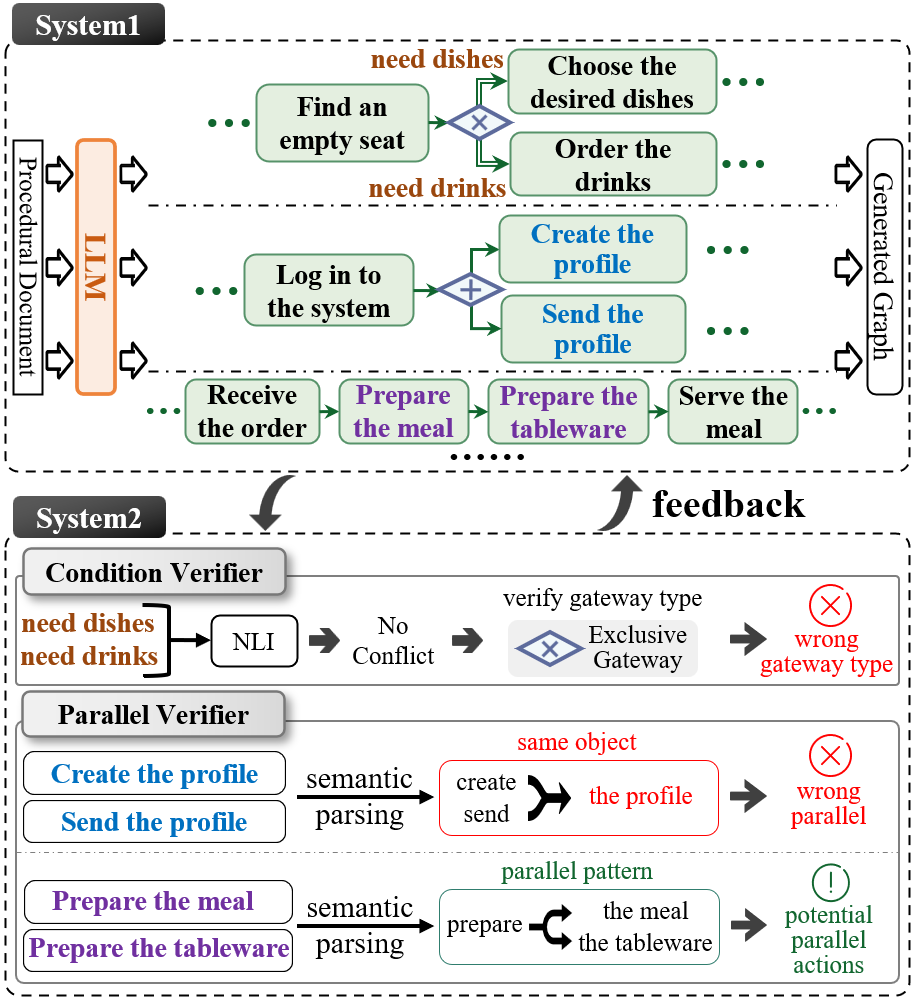
\includegraphics[width=\textwidth]{figures/Method.png}
    \caption{The proposed two-system based self-refine framework. 
    }
    \label{fig:method}
\end{figure*}

\subsubsection{Performance of LLMs}
% V1
% Despite the fact that large language models can outperform traditional methods by a large margin, they still can not solve this task well, especially for the extraction of gateways. 
% Additionally, we have the following observations:
% 1) It should be noticed that although end to end methods perform well in extracting most nodes, they are difficult to surpass traditional methods for exclusive gateways extraction except fine-tuned Llama2 model. This indicates that large models adopted by end to end approaches have trouble understanding complex branches in the documents and determine correct gateways to represent them. 
% 2) For End to End baselines, it is difficult for them to distinguish exclusive and inclusive gateways correctly. Although fine-tuned on training data, Flan-T5 and Llama2 still perform worse than ChatGPT for the extraction of inclusive gateways. This is because the amount of training samples containing exclusive gateways is larger than that containing inclusive gateways,leading the model to learn harmful biases and cannot correctly determine the use of exclusive and inclusive gateways. 
% Our proposed framework successfully corrects these biases through external feedback with the two-system based self-refine strategy. 
% 3) Llama2 fine-tuned model can outperform traditional methods for node, edge, and actor extraction by a large margin, even surpassing ChatGPT. This indicates that large-scale and high-quality training data is crucial for exploring effective procedural graphs extraction model. Flan-T5 model is fine-tuned on the train set but performs worse than Llama2 fine-tuned model. This is probably because the causal language model architecture is more efficient to utilize in-context learning mechanism compared to the seq2seq language model architecture adopted by Flan-T5 model. 
% 4) The performance of edge and actor extraction largely depends on the accuracy of node extraction, because without accurately extracted nodes, it is impossible to construct correct edges between nodes and extract corresponding actors of the action nodes. Therefore, the challenge of this task mainly lies in the accurate extraction of the nodes, especially the gateways used to represent complex branches. 
% 5) Pre-trained large language models bring new opportunities for the extraction of procedural graphs containing both procedural and factual knowledge. But further improvements are needed to deal with the accurate extraction of complex branches and the construction of edges between the extracted nodes. 

% V2
Despite the fact that LLMs outperform traditional methods for identifying actions, constraints and actors by a large margin, they still struggle to represent non-sequential actions. 
Additionally, we have the following observations:
1) It should be noticed that although end to end methods perform well in extracting most elements, they are difficult to surpass traditional methods for gateways extraction except fine-tuned Llama2 model. This indicates that LLMs have trouble understanding non-sequential execution of actions in the documents and use correct gateways to represent them. 
2) For End to End baselines, it is difficult for them to distinguish exclusive and inclusive gateways correctly. Although fine-tuned on train set, Flan-T5 and Llama2 still perform worse than ChatGPT for the extraction of inclusive gateways. This is because the amount of training samples containing exclusive gateways is larger than that containing inclusive gateways,leading the model to learn harmful biases and cannot correctly determine the use of exclusive and inclusive gateways. 
3) Llama2 fine-tuned model can outperform traditional methods for the extraction of all elements, even surpassing ChatGPT. This indicates that large-scale and high-quality training data is crucial for exploring effective procedural graphs extraction model. Flan-T5 model is fine-tuned on the train set but performs worse than Llama2 fine-tuned model. This is probably because the causal language model architecture is more efficient to utilize in-context learning mechanism compared to the seq2seq architecture adopted by Flan-T5 model. 

\subsubsection{Improvement Strategies}
Through our detailed analysis of the extracted graphs of the LLMs, we find that understand the non-sequential execution of actions and use correct gateways to represent them is challenging for LLMs. 
To alleviate this defect, inspired by the ``dual process'' theories~\cite{evans2003two}, we design a two-system based self-refine framework to verify the extracted graphs of the model and provide external feedback to refine the model's extractions. 
As shown in Figure~\ref{fig:method}, we adopt the LLM as ``System1'' to extract the procedural graphs from the documents. Then we design two verifiers as ``System2'' to verify the correctness of the extracted graphs and provide feedback to the model for further refinement if needed. 


\paragraph{Condition Verifier}
% We design a ``condition verifier'' to verify the correctness of the exclusive and inclusive gateways extracted by the model. The models often fail to distinguish between these two types of gateways.

% After careful analysis, we find that the essential difference between exclusive and inclusive gateways lies in whether there exists conflict between the conditions of different branches. 
% For exclusive gateways, once the condition of one specific branch is satisfied, the conditions of other branches must not be satisfied, that is, all conditions of a single exclusive gateway are mutually ``exclusive''. 
% On the other hand, there exists no conflict between the conditions of a single inclusive gateway, that is, more than one conditions of the inclusive gateway can be satisfied at the same time. 

% Inspired by this, we design a simple and effective verifier to detect the conflict between the conditions of the branches and verify the correctness of corresponding gateways. 
% We adopt the off-the-shelf Natural Language Inference (NLI) model to measure the conflict between two conditions. If the conflict is detected for a inclusive gateway or no conflict is detected for an exclusive gateway, we will provide the feedback to the model. The model will further refine its predictions based on the provided feedback. 

The model often fails to distinguish between exclusive and inclusive gateways. 
After careful analysis, we find that the essential difference between exclusive and inclusive gateways lies in whether there exists conflict between the conditions need to be satisfied. 
Inspired by this, we design a simple and effective verifier to detect the conflict between the conditions of the extracted exclusive and inclusive gateways with off-the-shelf Natural Language Inference model, and provide the feedback to the model if: (1) a conflict is detected for inclusive gateways or (2) no conflict is detected for exclusive gateways. 
For example, the model extracts an exclusive gateway with conditions ``need dishes'' and ``need drinks'' that are not conflicted, and the verifier then provides feedback to the model for correcting the gateway type. 

\paragraph{Parallel Verifier}
% We design a ``parallel verifier'' to verify the correctness of the parallel branches predicted by the model and explore potential parallel branches that may have been missed by the model. 

We find that different actions can be executed in parallel only when the objects of these actions are different. On the contrary, if several actions are executed on a same object, they cannot be executed in parallel. 
Inspired by this, we design a verifier to verify the objects difference for parallel actions through semantic parsing. Additionally, we further explore the actions executed in sequence but on different objects, especially for those that meet the special syntactic pattern of ``same predicate with different objects'', which are capable of the potential for parallel execution and often neglected by the model. 
For example, two sequential actions ``prepare the meal'' and ``prepare the tableware'' have same predicate ``prepare'' and different objects, and the verifier then provides feedback to the model for extracting this potential parallel gateway. 

\begin{figure}[h]
    \centering
    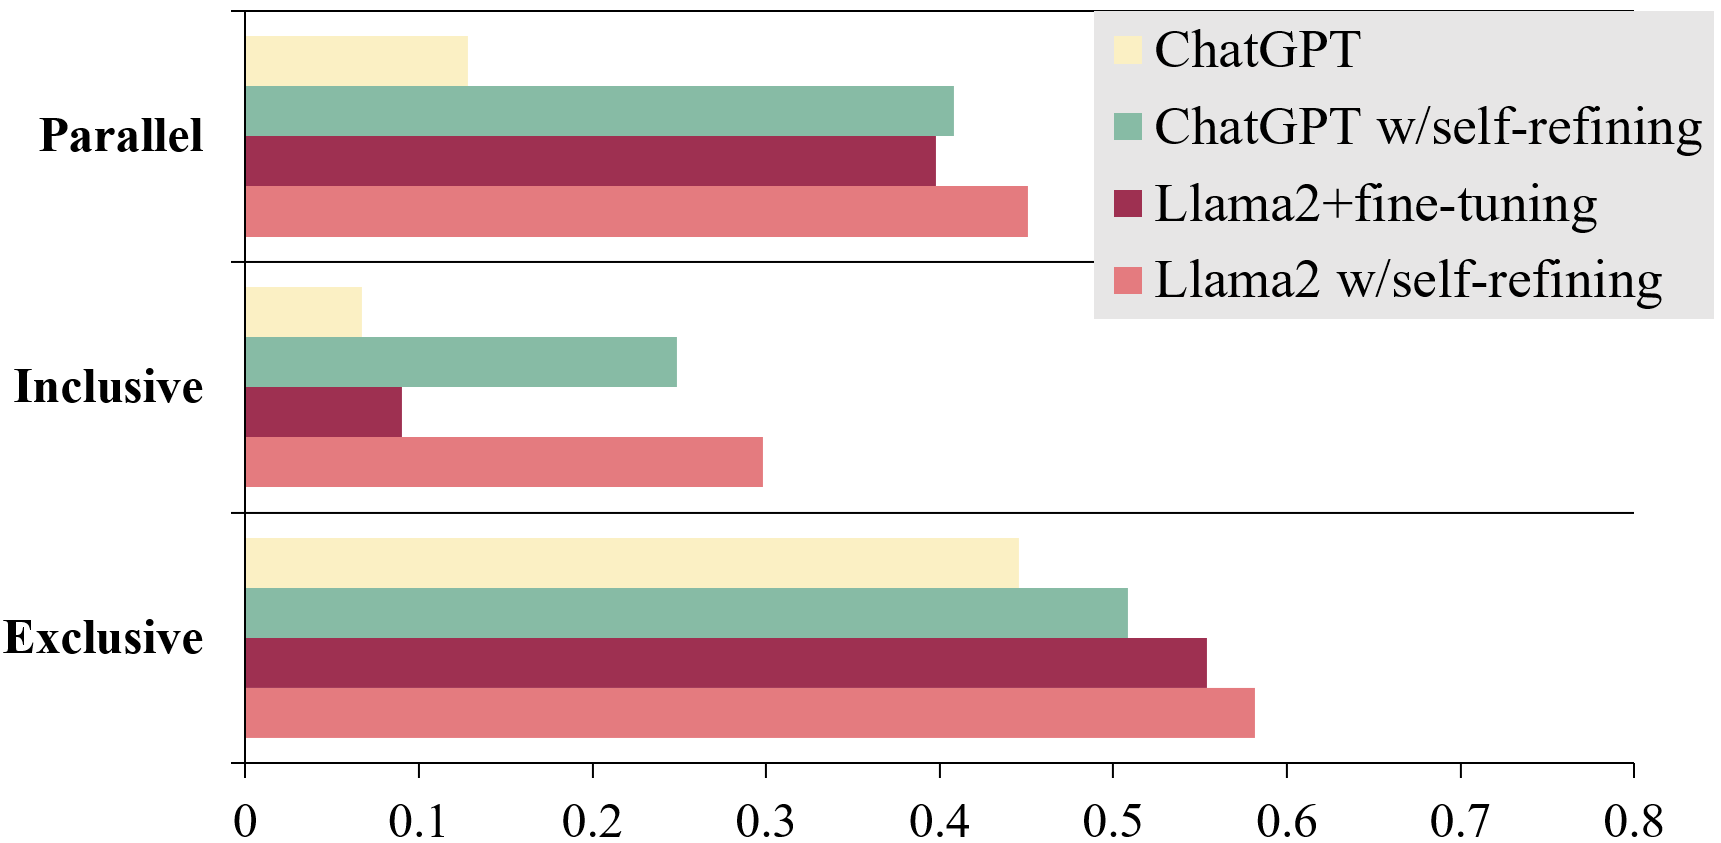
\includegraphics[width=\linewidth]{figures/improve.png}
    \caption{Results of proposed improvement strategies and corresponding baseline models.
    }
    \label{fig:improve}
\end{figure}

% \begin{table}[]
\caption{Results of proposed framework and corresponding baseline models. Best results are represented in bold.
}
\label{tab:improve}
\centering
\scalebox{0.9}{
\begin{tabular}{|l|c|c|c|}
\hline
\multicolumn{1}{|c|}{\textbf{Model}} & \textbf{XOR}    & \textbf{OR}     & \textbf{AND}    \\ \hline
ChatGPT                              & 0.4459          & 0.0672          & 0.1284          \\ \hline
Llama2 fine-tuned                    & 0.5539          & 0.0900          & 0.3979          \\ \hline
self-refined ChatGPT                 & 0.5085          & 0.2487          & 0.4081          \\ \hline
self-refined Llama2                 & \textbf{0.5814} & \textbf{0.2983} & \textbf{0.4511} \\ \hline
\end{tabular}
\vspace{-0.3cm}
}
\end{table}



\paragraph{Results}
% imporvement of strategies
As shown in Figure~\ref{fig:improve}, with the assistance of our proposed strategies, both ChatGPT and Llama2 achieve significant performance improvements for gateways extraction. This is because our proposed strategies help the model correctly understand the non-sequential actions in the documents and use correct gateways to represent them through external feedback provided by our designed verifiers. 
This indicates that the main challenge of utilizing LLM for optimal procedural graphs extraction lies in the comprehension and representation of non-sequential actions. 


% \paragraph{Self Refine}
% We provide feedback obtained from the two verifiers in ``System2'' to ``System1'' and promote the model in ``System1'' to refine the extracted graphs based on the feedback. 
% Due to space limitations, the specific templates used to generate the feedback are presented in the appendix. 

\subsection{Model Capabilities Analysis}
As shown in Figure~\ref{fig:Radar}, we divide the capabilities required for the extraction of optimal procedural graphs into seven dimensions and conduct comparison between several representative models to show their capabilities in different dimensions. 
We can see that compared with traditional methods, ChatGPT has greatly improved the capabilities in most dimensions, but there is no significant progress for gateway extraction. This indicates that even the powerful LLMs struggle to understand non-sequential actions in the documents. PET utilizes labeled training data to achieve improvement for action extraction compared to Translation Like model, but still performs poorly for gateway extraction. This is because the labeled data used by PET only contains individual action annotations and cannot help the model to learn represent non-sequential actions with correct gateways. Self-refined Llama2 alleviates these defects by fine-tuning on our constructed dataset and utilizing our proposed strategies. 
In general, existing solutions are still unable to accurately extract optimal procedural graphs from the documents, and the main challenge lies in the extraction of non-sequential actions. 

\begin{figure}[h]
    \centering
    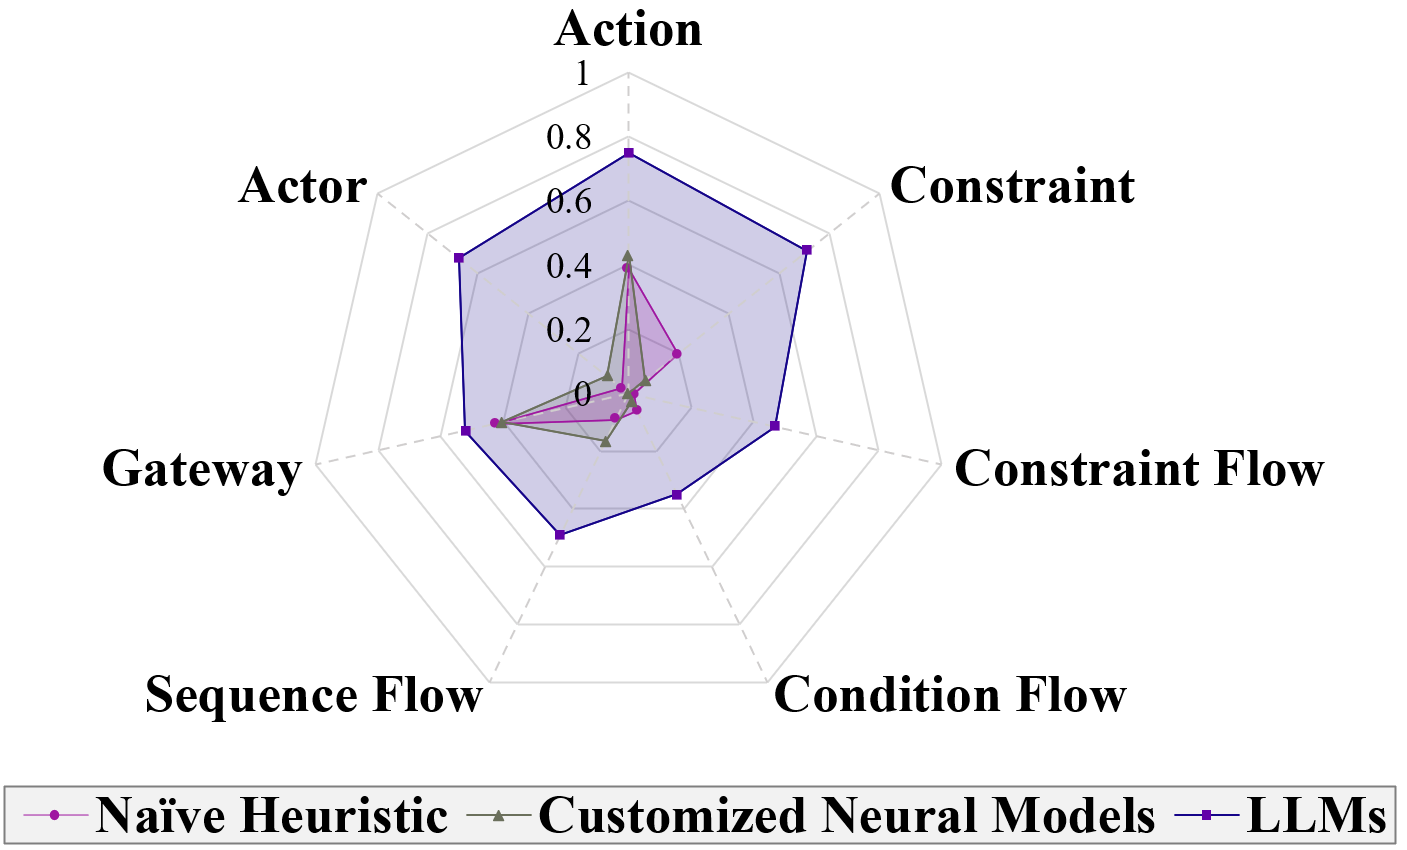
\includegraphics[width=8cm]{figures/Radar.png}
    \caption{Comparison of capabilities between several representative models. ``Gateway'' dimension represents the extraction of the three types of gateways. 
    }
    \label{fig:Radar}
\end{figure}

% advantages of various models and the challenges of this task

\subsection{Case Study}

\begin{figure}[h]
    \centering
    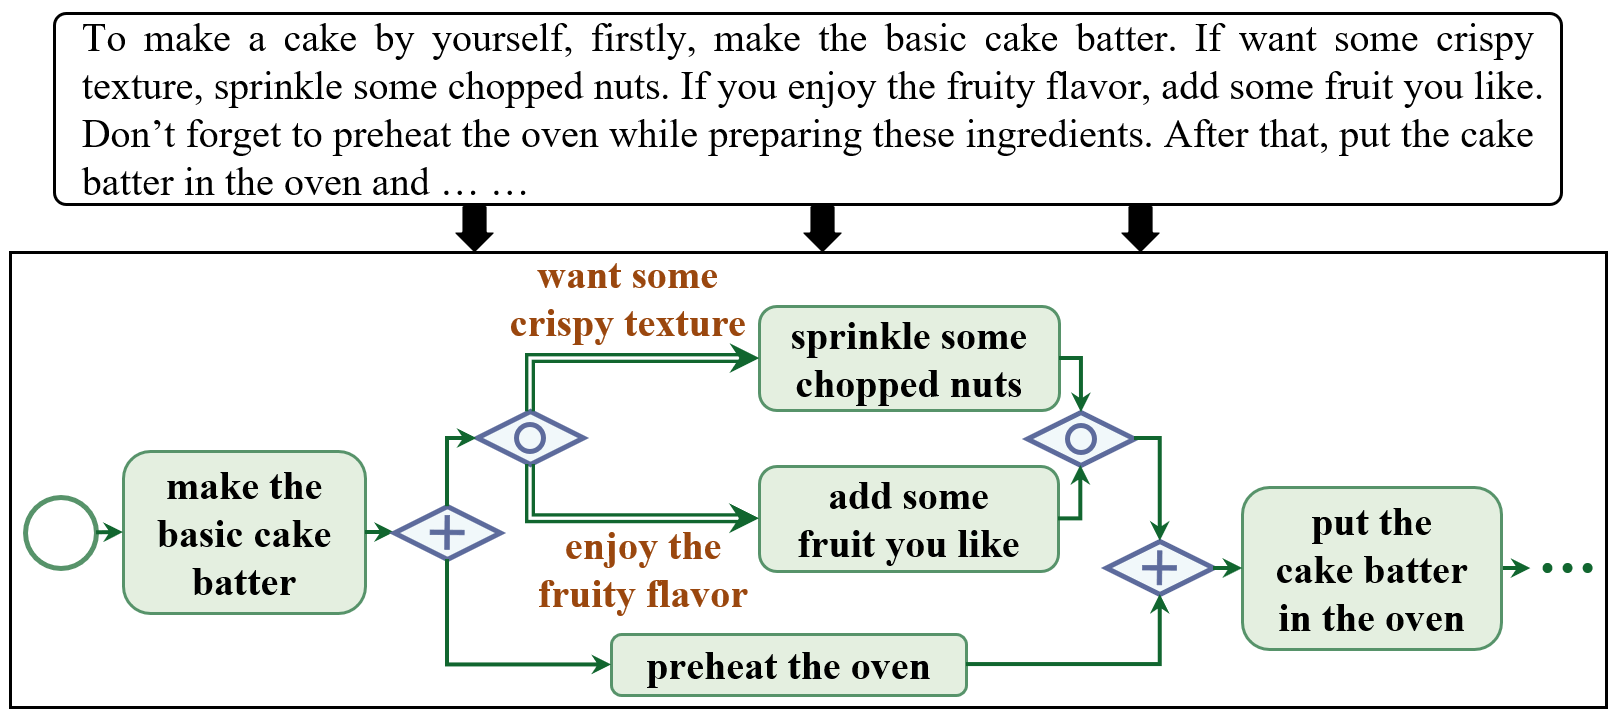
\includegraphics[width=0.5\textwidth]{figures/Case.png}
    \caption{An example of the partial procedural graph extracted by our proposed framework from the document.
    }
    \label{fig:Case}
\end{figure}
As shown in Figure~\ref{fig:Case}, LLM with our proposed strategies can accurately extract complex non-sequential actions from the document, even in cases where different types of gateways are nested within each other. Through the feedback provided by our designed verifier, the model successfully understands that there exists no conflict between the two conditions "want some critic texture" and "enjoy the freedom lover", and correctly use the inclusive gateway to represent the non-sequential actions. 
Meanwhile, thanks to the strong semantic understanding ability of the LLM, it successfully identifies and extract the parallel actions hidden in the document. 

